
\documentclass[11pt]{article}
\usepackage{graphicx}%
\usepackage{caption}
\usepackage{subcaption}
\usepackage{float}

\setlength{\oddsidemargin}{0in} \setlength{\evensidemargin}{0in}
\setlength{\textwidth}{6.5in} \setlength{\topmargin}{0in}
\setlength{\headsep}{0in} \setlength{\parskip}{0.1cm}
\pagestyle{plain} \setlength{\textheight}{9.0in}
%end of preamble
\renewcommand{\baselinestretch}{1.0}
\newcommand{\be}{\begin{equation}}
\newcommand{\ee}{\end{equation}}
\newcommand{\bea}{\begin{eqnarray}}
\newcommand{\eea}{\end{eqnarray}}
\newcommand{\nn}{\nonumber}
\newcommand{\bd}{\begin{description}}
\newcommand{\ed}{\end{description}}
\newcommand{\bc}{\begin{center}}
\newcommand{\ec}{\end{center}}
\newcommand{\mysection}[1]{\vspace{.05in} \noindent {\bf  #1}\\ \indent}
\newcommand{\mysubsection}[1]{\vspace{0in} \noindent {\bf #1}\\ \indent}
\newcommand{\mynotationsubsection}[1]{\vspace{.05in} \noindent {\bf #1} \indent}
\newcommand{\myreferencessection}[1]{\vspace{.05in} \noindent {\bf #1} \indent}
\newcommand{\mysubsubsection}[1]{\vspace{.05in} \noindent {\bf #1}\\ \indent}
\renewcommand{\baselinestretch}{2}

\begin{document}
\begin{center} Managing Projects with Uncertain Deadlines
\end{center}
%\begin{center}
%Robert F. Bordley, Professor and Program Director, University of Michigan Ann %Arbor, rbordley@umich.edu \\
%Jeffrey M. Keisler, Professor, University of Massachusetts Boston, Boston, MA %02125, jeff.keisler@umb.edu \\
%Tom M. Logan, University of Michigan, Ann Arbor, MI 48109, tomlogan@umich.edu
%\end{center}
\begin{abstract}
In conventional project management, the project manager is given a deadline and is responsible for making decisions assuming this deadline will not change. But in reality, project deadlines frequently change.  Conventional project management addresses unanticipated changes in the project deadline with external change control processes.  If this external process changes the deadline, the manager will replace the original deadline with the modified deadline.  The manager is still supposed to assume this modified deadline is fixed in making project decisions.\par  As this paper will show, recognizing deadline uncertainty can substantially improve the value of the manager's decisions.  Deadline uncertainty could be formally addressed in project management by making dramatic changes in conventional project management.  But given the widespread use of project management, making such dramatic changes might not be feasible.  This paper presents a much more easily implemented approach to incorporating deadline uncertainty into managerial decision making which makes no changes to conventional project management procedures. \\
\bf Key Words: \rm Decision Analysis, Project management, Project scheduling, Uncertainty modelling
\end{abstract}
\section {Introduction}
         Project management (Kerzner, 2009; Meredith and Mantel, 2003) is a management discipline receiving continuously growing attention and being applied in an increasing number of organizations (Leus, Wullink, Hans and Herroelen, 2003).  Project management creates deliverables for its stakeholders by identifying and managing the various project activities that must be completed in order to create these deliverables.   A large portion of project management practice is based on what we shall term conventional project management heuristics (Klastorin, 2003; Project Management Institute, 2013; Miller, 1963).  These heuristics are described in the project management book of knowledge (PMBOK) which is the basis for the certification of more than $800,000$  active project management professionals (PMP) in $210$ countries. \par 
         Project management involves defining the scope of the project, the project stakeholders and the project deliverables, budget and deadline. The next step is identifying all the work activities which must be completed in order to achieve the project's deliverables.  Precedence relationships are then identified which specify which activities must be completed before others can start.    Based on these precedence relationships, activities are arranged in a project network which is a directed acyclic graph. (Design structure matrix methods (Eppinger and Browning, 2012) help ensure the graph is acyclic.)  A path through this network is a sequence of consecutive activities with the completion time of a path being the sum of the completion time of the activities along that path.  There are typically multiple overlapping paths in the network. The project finishes when the path with the longest completion time (also known as the critical path) finishes. \par The critical path method (CPM) focuses on reducing project completion time by `expending extra resources on activities on the critical path' or transferring resources from non-critical paths to the critical path.  CPM assumes there is no uncertainty in the duration of any of the activities (and thus no uncertainty in the completion time of any of the project's paths.)  The performance evaluation and review technique (PERT) and the graphical evaluation and review technique (GERT) generalize CPM by recognizing uncertainty in the time needed to complete the various project activities (Kamburowski, 1996; Sculli, 1989; Golenko-Ginzburg, 1989). This creates uncertainty about which path finishes last.   PERT resolves this uncertainty by defining the critical path to be the path with the greatest mean completion time. PERT also uses beta distributions to describe the uncertainty in activity completion times and normal distributions to describe the uncertainty in path completion times.  There are other ways e.g., decision analytic methods, for specifying an activity's completion time (Keefer and Verdini, 1993), as well as other more flexible alternatives to the beta distribution (Perez, Martin, Garcia and Granero, 2016).
         GERT allows for more general distributional assumptions and project networks than PERT.  However GERT still presumes that the project's stakeholders have specified definite (i.e., certain) requirements for the overall project's completion time at the start of the project. This is also true for other risk-based project management approaches (Zafra-Cabeza, Ridao and Camacho, 2008; Herroelen and Leus, 2003; Herroelen and Leus, 2005).  \par
         But it is well known that requirements change because of unforeseen changes in stakeholder needs (Ward and Chapman, 2003; Huemann, Turner and Keegan, 2007; Bordley and Keisler, 2015) or because certain activities either fail to achieve (or over-achieve) their requirements.   
         As a result, project management provides a change control process which can change the project's deadline (as well as other requirements) after the start of the project.  This process is reactive in requiring the project manager to treat the deadline as fixed --- until such time as a change control process adjusts the deadline and leads to a change in project plan (Calhoun, Deckro, Moore, Chris and Hove, 2002). But while this change control process reduces some of the disruption caused by specification changes,  change is still disruptive and typically requires that some previous work be redone or discarded. \par To reduce the amount of rework, agile approaches (Maylor,  Vidgen and Carver, 2008) attempt to restructure the work flow so that the project manager does not start work on certain activities until the requirements for those activities are known. If stakeholder understandings of their own requirements deepen as the deliverable is developed, then agile approaches can mitigate the uncertainty associated with stakeholders changing their requirements.   But it requires more frequent iterations with the stakeholders which can be costly and time-consuming (Schwaber, 2004). Agile also does not address those changes in the requirements for later activities which arise because current activities fail to achieve or over-achieve their requirements. To respond quickly to these kinds of changes,  techniques such as active monitoring and corrective action (Hu,Cui, Demeulemeester and Bie, 2016), or generation of options (Creemers, De Reyck and Leus, 2015) are used.
         \par
          Both the conventional and agile approaches to project management still require the project team to treat requirements as fixed (and certain) until they are officially changed. But a manager who recognizes requirement uncertainty will often make higher quality and more robust decisions than a manager who ignores requirement uncertainty.   As Morgan and Henrion (1982) note, the expected value of including uncertainty can be substantial.  There are, of course, a wide variety of decision tools that can already be used for decision making under uncertainty (Ding and Zhu, 2015; Elmaghraby, 2003; Morgan and Henrion, 1992;  Chapman and Ward, 1997; Clemen, 1996; Khodakarami, Fenton and Neil, 2007; Pich, Loch and DeMeyer, 2002).  
Many of these common decision analysis methods are already recognized in the PMBOK and are often use by the project manager in addressing uncertainty associated with the duration, cost and feasibility of various activities in the project. But these methods have not been used to address requirement uncertainty.   \par
The focus of this paper is on deadline uncertainty, whose importance is highlighted by the substantial research on make-span minimization (Kolish and Padman,2000).    As we show, a project with uncertain activities and an uncertain deadline is equivalent to a project with an additional uncertain activity and a fixed deadline.  Introducing this additional activity is consistent with an established project management tradition of introducing fictitious or dummy activities with zero expected duration to the activity network (e.g., Neumann and Zimmerman, 1999; Estevez-Fernandez, 2012).  In our approach, this additional activity will have an uncertain non-zero duration. With this additional activity, the same techniques currently used for managing projects with uncertain activities can be used for managing projects with both uncertain activities and  deadlines. \par
The next section presents this solution to the problem of accounting for deadline uncertainty in project planning. To establish the value of this solution, the third section shows how ignoring deadline uncertainty underestimates the schedule risk associated with each path in the project.  This can mislead the manager into mis-allocating resources across the project's activities.  The fourth section calculates bounds on the improvement in project on-time completion probability when deadline uncertainty is considered. Project on-time completion probability will depend on the complex  interdependencies between paths in the project.
The fifth section conducts a designed experiment involving a thousand randomly generated projects in order to quantify the improvement provided by this solution. The sixth section shows that the benefits of our approach are not contingent on any of the controversial assumptions associated with conventional project management heuristics.  
\section{Proposed Conceptual Solution}
\subsection{Motivation}
First consider the following motivating example. Suppose the stakeholder, upon receiving the deliverables from the manager's project, immediately starts a 'complementary' activity designed to use those deliverables to finish some longer term project.  When the manager's project and this complementary activity are finished, the longer-term project is finished (See Figure 1).   Suppose the longer-term project has a fixed required completion time $r_O$.   If the completion time of the complementary activity were known to be $t$, then the stakeholder could give the manager's project a fixed deadline of $r=r_O-t$ which would then allow the stakeholder to meet their deadline of $r_O$. \par
But suppose the completion time of the complementary activity is uncertain. Then the required completion time, $r$, for the manager’s project will be uncertain.   So the stakeholder cannot give the manager a fixed deadline for the original project.\par
\begin{figure}[ht]
\begin{center}
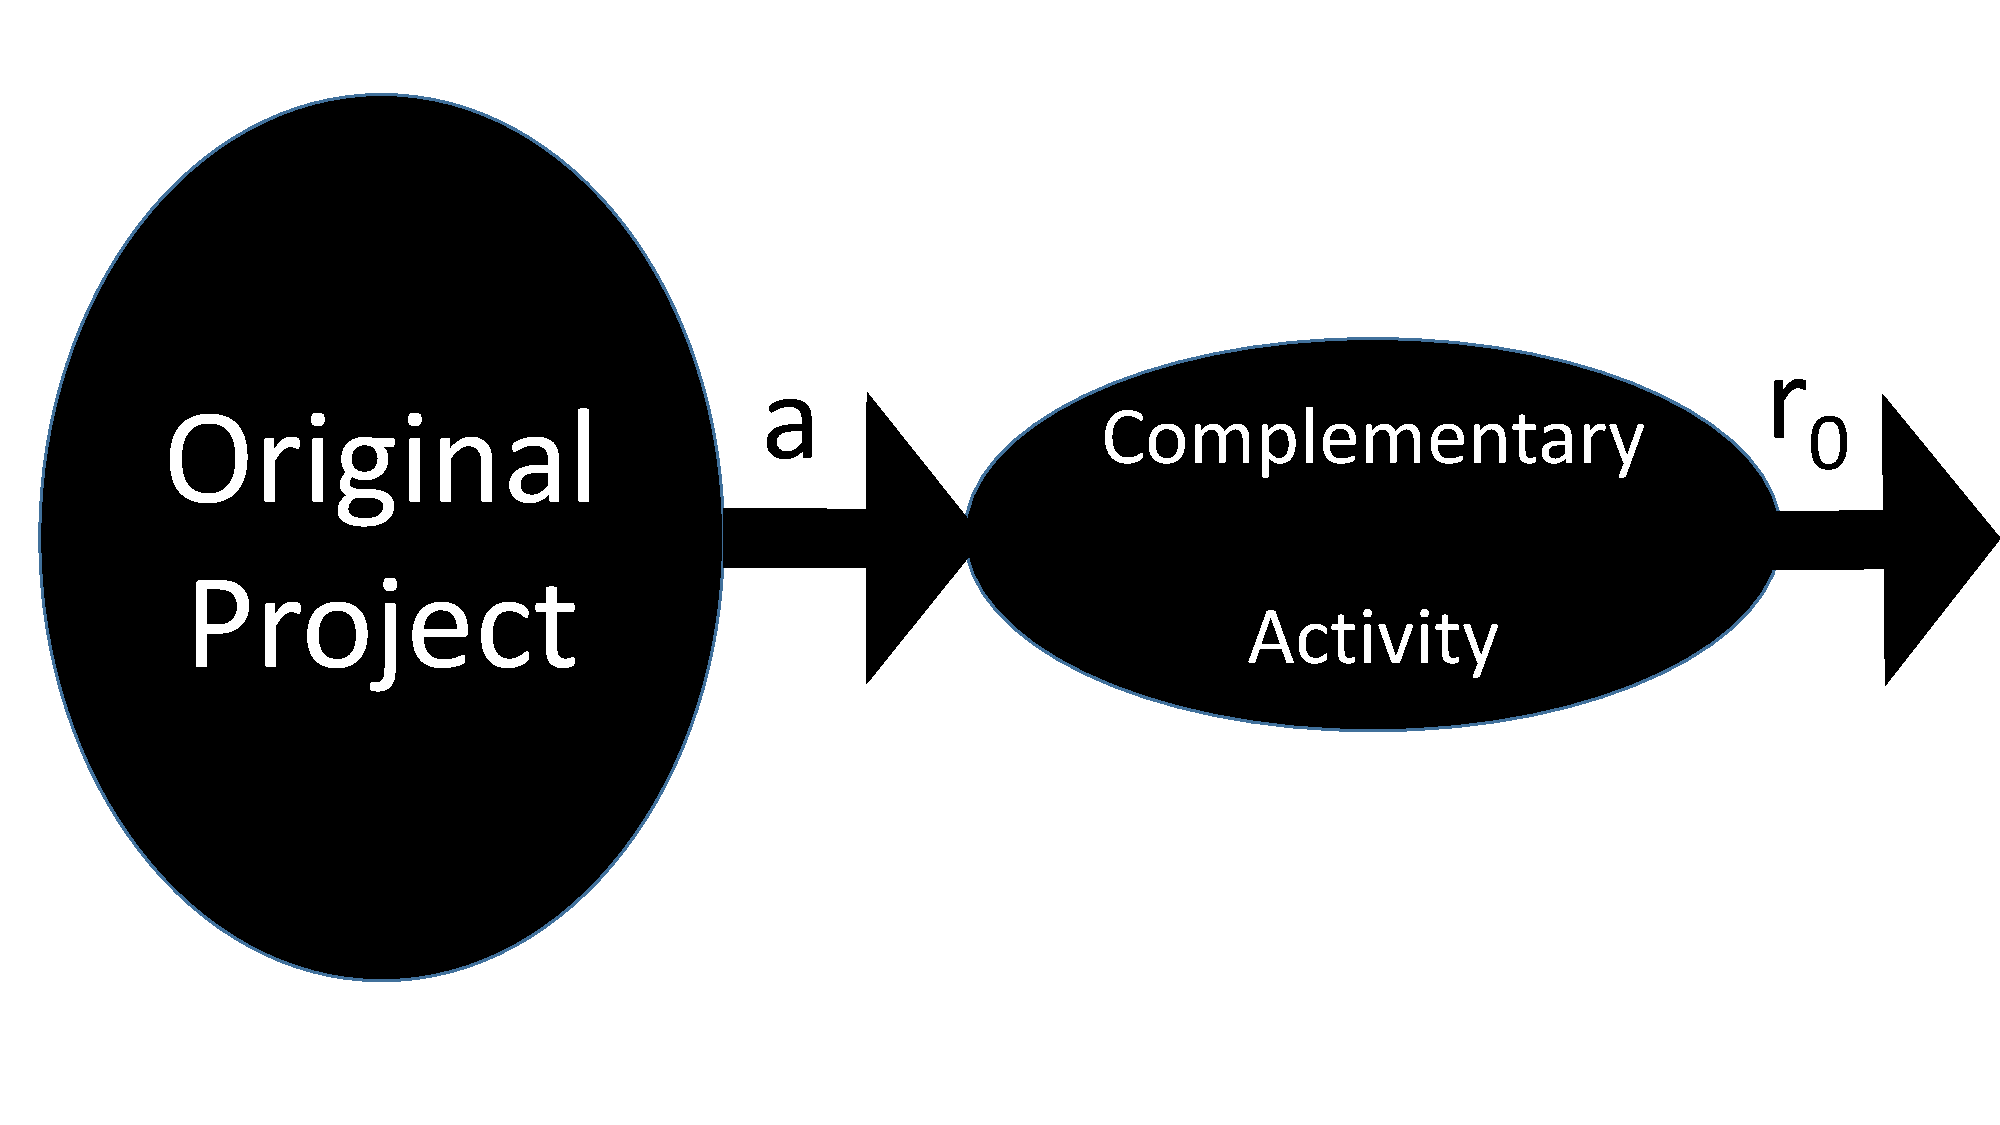
\includegraphics[scale=0.30]{uncertaindeadlines.pdf}
\caption{The Original Project embedded in the Manager's Project}
\label{fig:orginalproject}
\end{center}
\end{figure}
          Fortunately, the manager could simply re-define the actual project so that it finishes when the longer term project finishes.    This enlarged project will have the same required completion time $r_O$ as the stakeholder's long-term project.   The project network describing the new project consists of the network for the original project plus an additional activity, corresponding to the complementary activity, which can only start after all the activities in the original project have finished.  But while the manager may be able to affect the completion time of the activities in the original project by adding resources, the manager will not be able to affect the completion time of this complementary activity. \par
          If the completion time of the complementary activity is $t$ and if the actual completion time of the manager's project is $a$, then the completion time for the redefined project will be $a+t$.   The project will finish on time when $a+t \leq r_O$.   Since PERT describes the uncertainty in each activity's duration using optimistic, pessimistic and most likely estimates, the manager could similarly describe the uncertainty in $t$ by specifying an optimistic completion time, $t_O$, for the complementary project, a pessimistic completion time $t_P$  and a most likely completion time, $t_L$.  The manager could then use standard PERT methods to model the probability of the redefined project finishing by its new deadline $r_O$ (which is just the probability that $a+t \leq r_O$.)   The uncertainty in the deadline of the original project is completely determined by the uncertainty in the complementary activity.   (The uncertainty in the actual completion time, $a$, of the original project is, of course, described by the uncertainty in the activities within the original project.)  Since the manager is now responsible for a redefined project including the complementary activity, the manager will make decisions that appropriately consider the uncertainty in the required completion time for the original project.
\subsection{Extension to General Projects}
          We now show how the solution for the special case just described can be extended to the more general case where there is no longer-term project but the stakeholder is still uncertain about the time when the project must finish.  Let $r_O$, $r_L$ and $r_P$ be the stakeholder's estimate of the latest possible project deadline, the most likely project deadline and the earliest project deadline.  Define $t=r_O-r$ where $r$ is the uncertain required completion time for the project.  Then $t$ will have a maximum possible (pessimistic) value of  $t_P = r_O-r_P$ , a most likely value of  $t_L = r_O-r_L$ and a minimum (optimistic) value of   $t_O = r_O-r_O=0$.  The manager's project will finish on time if $a < r $ (which implies $a+t < r_O$. )  Hence, making decisions to maximize the probability of $a+t$ being less than $r_O$ will be equivalent to making decisions to maximize the probability of the original project having a completion time, $a$, which is earlier than its original uncertain deadline, $r$.  \par
          To model this with the classical project management activity network, the manager re-defines the original project to have a deadline $r_O$ and to include a fictitious complementary activity with uncertain completion time $t$ which starts when all other activities finish.   Fictitious activities have been used, for other purposes, in other project management contexts (Vanhoucke (2013), pg. 244; Schwindt (2005), pg.8).  The classical project management solution to the original project supplemented with this added activity will be the appropriate solution to the original project where the stakeholder's completion time was uncertain.\par
          \section{Path On-Time Completion Time}
          \subsection{Overestimation of on-time path completion probability}
Number the paths $i=1...k$. Let $X_i$ represent the uncertain completion time of path $i$ with $T$ representing the uncertain deadline.  This paper will use the term slack to describe $T-X_i$ which is the uncertain amount by which path $i$ finishes ahead of the deadline.  Let $X_i$ and $T$ have variance $v_i$ and $v$ respectively.  Let $e_i$ be the mean of the uncertain slack.  Then the variance of the slack is $v_i+v$ if deadline uncertainty and path uncertainty are uncorrelated. (The argument can be extended to allow for correlation.)
The probability of path $i$'s on-time completion is
$$ p_i = P(X_i \leq T) = P(T-X_i \geq 0) = P(\frac{T-X_i-e_i}{\sqrt{v_i+v}} \geq - \frac{e_i}{\sqrt{v_i+v}})  =
P(\frac{e_i-(T-X_i)}{\sqrt{v_i+v}} \leq \frac{e_i}{\sqrt{v_i+v}})  $$
Define
$$
\eta_i = \frac{e_i-(T-X_i)}{\sqrt{v_i+v}} \mbox{ and }
z_i = \frac{e_i}{\sqrt{v_i+v}}  $$
and let
$F_i$ be the cumulative distribution of the standardized random variable $\eta_i$.  Then $p_i=P(\eta_i \leq z_i)=F_i(z_i)$.  
While this paper requires $F_i$ to be continuous with probability density $f_i$, it does not require $F_i$ to be the standard normal distribution used in PERT analysis.   Thus the standardized skewness, kurtosis and other moments associated with path $i$ need not equal the standardized moments for the normal distribution (or even the corresponding standardized moments for other paths.) 
\par   
Suppose the manager who ignores the variance in the deadline estimates the deadline $t$ as the mean of $T_i$.  Then the mean value of $t-X_i$ is still $e_i$ but the variance is $v_i$ instead of $v_i+v$. The manager will estimate the probability of path $i$ finishing on-time as 
$$ p^0_i= P(\frac{e_i-(t-X_i)}{\sqrt{v_i}} \leq \frac{e_i}{\sqrt{v_i}})  $$
If $\eta^0_i=\eta_i|_{v=0}$ and $z^0_i=z_i|_{v=0}$, then $p^0_i=F_i(z^0_i)$.\par 
If there were no uncertainty in the project or the deadline, then the project manager should set the deadline so that it equals or exceeds the completion time of every path.  When there is uncertainty, this motivates:
\\
\bf Assumption 1: \rm The expected deadline equals or exceeds the expected completion time of path $i$ and $e_i \geq 0$. \\ 
Given this assumption,   $z_i \leq z^0_i$ and $$p_i=F_i(z_i) \leq F(z^0_i)=p^0_i.$$ 
As deadline uncertainty, $v$, increases, $p^0_i-p_i$ increases. As $v \Longrightarrow \infty$, $e_i \Longrightarrow 0$ so that $p^0_i = F_i(0)$.  \par
Now suppose that \\
\bf Assumption 2: $-\eta_i$ is unimodal and skewed to the right.\\
\rm Then the mode of $-\eta_i$ is less than the median which is less than the mean (Levin and Fox,2003).  Hence the mean of $\eta_i$ (or zero) is less than the median and $p^0_i=F_i(0)< 0.5$. As a result, extreme deadline uncertainty reduces the on-time completion probability of the path to $50\%$ or less.\par
This result does not specify how quickly $p^0_i$ converges to $50\%$.  To examine convergence, Figure \ref{fig:overestimate} plots $F_i(z_i)-F_i(z^0_i)$ as a function of deadline variance for the normal distributions.
\begin{figure}[ht]
\begin{center}
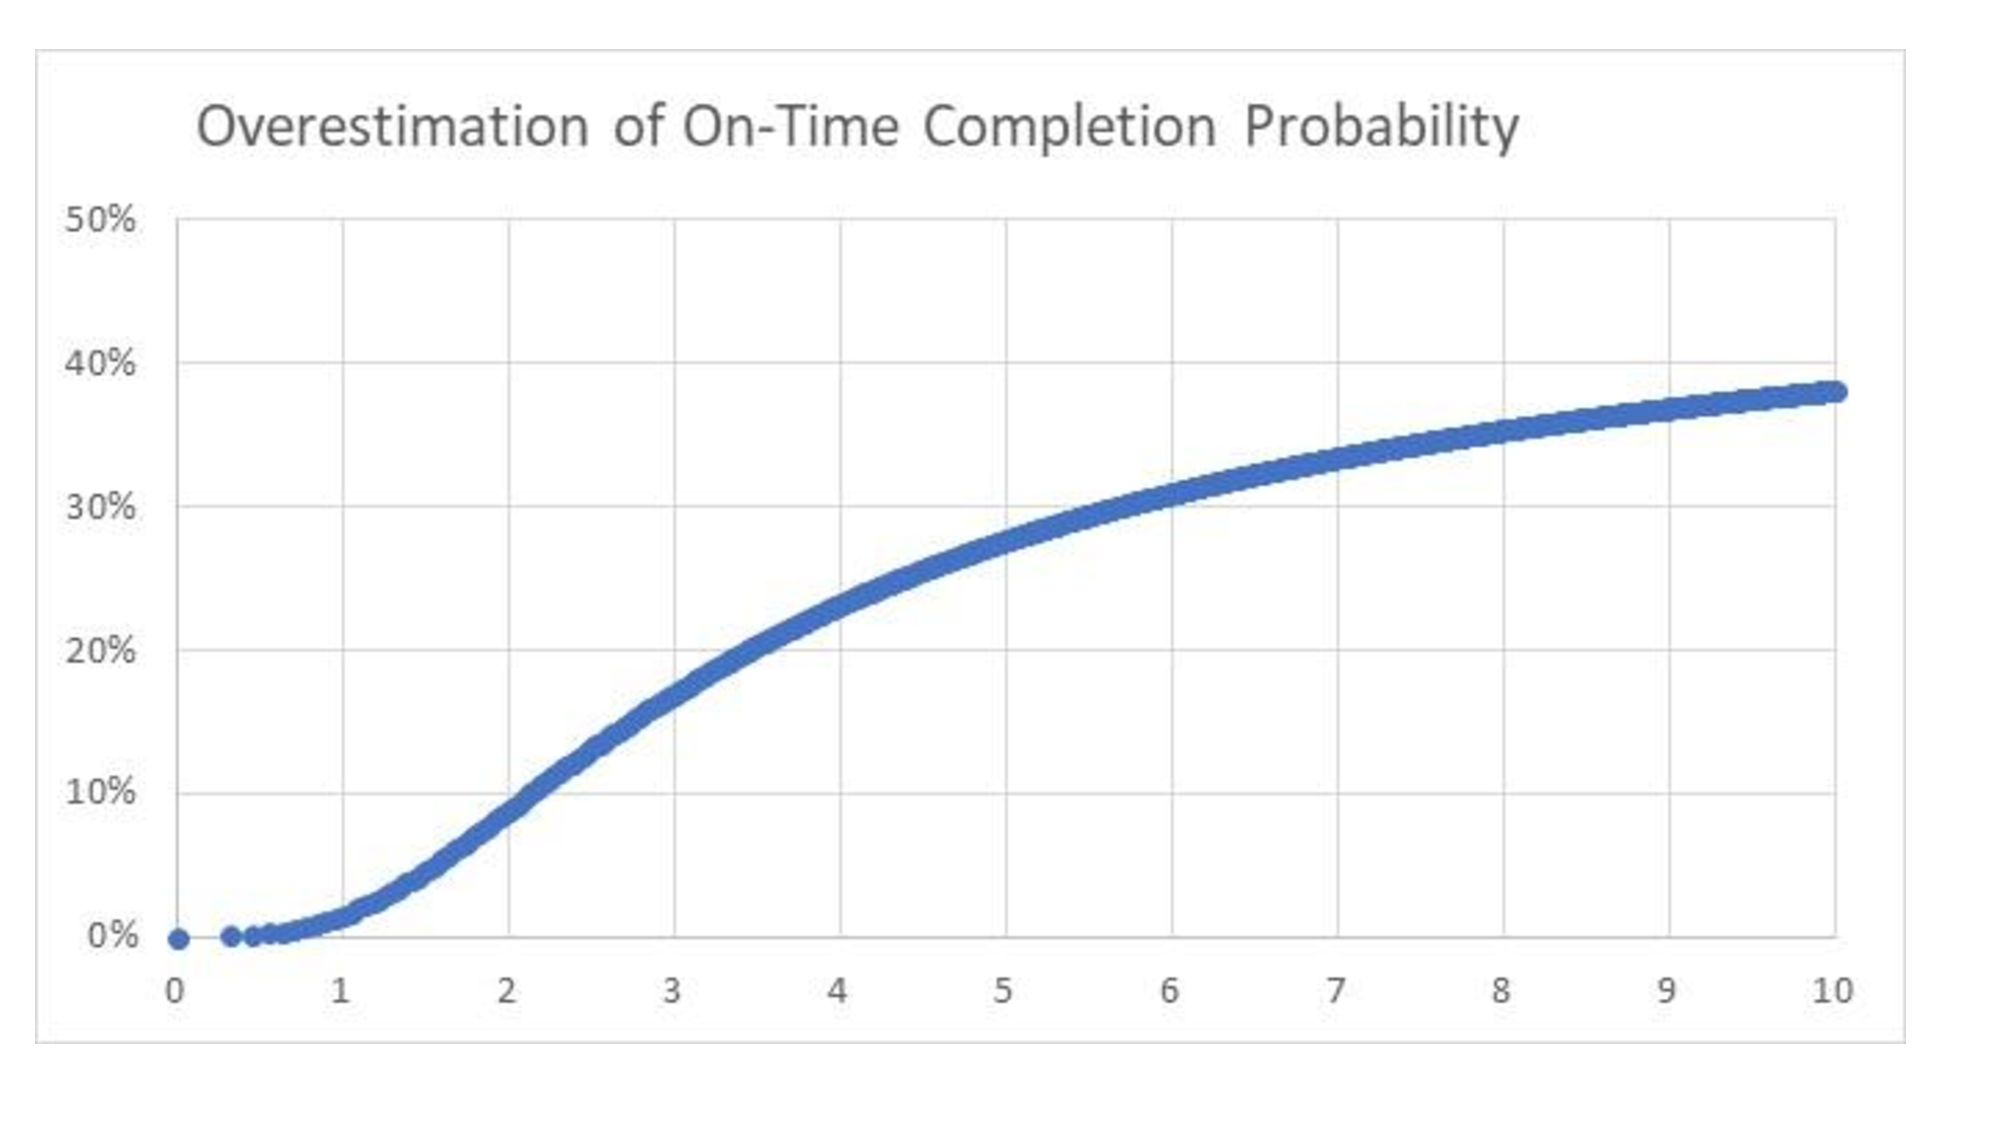
\includegraphics[scale=0.30]{projectmanagementdeadlineuncertaintyoverestimation.pdf}
\caption{Overestimation of on-time path completion probability with deadline standard deviation}
\label{fig:overestimate}
\end{center}
\end{figure}
To extend this result to non-normal distributions, let $p'_i$ and $p''_i$ be the first and second derivative of $p_i=F_i(\frac{e_i}{\sqrt{v+v_i}}) $ with respect to $v$.  Then we can expand $p_i$ in a Taylor Series about $v=0$.  The first-order Taylor Series approximation is
$$p_i -p^0_i= v p'_i |_{v=0} =p^0_i- \frac{1}{2} v [f(\frac{e_i}{\sqrt{v+v_i}}) \frac{e_i}{(v+v_i)^{3/2}}]|_{v=0}
\Longrightarrow
p^0_i-p_i = \frac{v}{v_i} z^0_i f_i(z^0_i)  $$
which is larger for low-variance paths (paths with smaller $v_i$).  This is consistent with what was observed when the slack was Gaussian. \subsection{Impact of Overestimation on Resource Allocation}
Suppose there is some initial allocation of resources to activities during the project.  If the manager wishes to shorten an activity's duration, the manager can adjust by allocating additional resources to certain activities (or `crashing' those activities). Suppose the manager considers the path with highest schedule risk (and lowest on-time completion probability) and adds resources to the activity in order to improve its on-time completion probability to some threshold value $\alpha$ (which might be the on-time completion probability of the path with the next highest schedule risk.)  If the manager can only change the mean completion time of activities in the project, then the manager needs to add sufficient resources to adjust $e_i$ to some value $e^*_i$ for which $F(\frac{e^*_i}{\sqrt{v_i}})=\alpha$. 
If $F_i$ is invertible, then $e^*_i=\sqrt{v+v_i} F^{-1}_i(\alpha)$.  But if deadline variance is ignored, the manager will set $e_i$ to $$e^0_i = \sqrt{v_i} F^{-1}_i (\alpha) = e^*_i \sqrt{\frac{v_i}{v+v_i}} 
= \frac{e^*_i}{\sqrt{1 + \frac{v}{v_i}}} \leq e^*_i  $$
so the manager allocates insufficient resources to crashing.  Substituting this insufficient value into the correct formula for on-time completion probability gives
$$\alpha^0=F_i(\sqrt{\frac{v_i}{v+v_i}} F^{-1}_i(\alpha)) $$
which is less than $\alpha$.   The difference $\alpha-\alpha_0$ is a function of $\frac{v}{v_i}$ and converges to $F(0) \leq 0.5$ as $v$ increases.  
\par
\subsection{Impact of Crashing on Different Paths}
The previous subsection focused on how ignoring deadline uncertainty misleads the manager into insufficiently resourcing a project path.  Figure \ref{fig:p_vary_uncertainty} considers a low-variance and high-variance path and shows that  deadline variance distorts the completion time of the low-variance path more than the completion time of the high-variance path.  (Both path completion times are assumed Gaussian for illustrative purposes.)   As a result, a manager who neglects deadline variance is biased toward crashing lower-variance paths.  
 \begin{figure}[ht]
\begin{center}
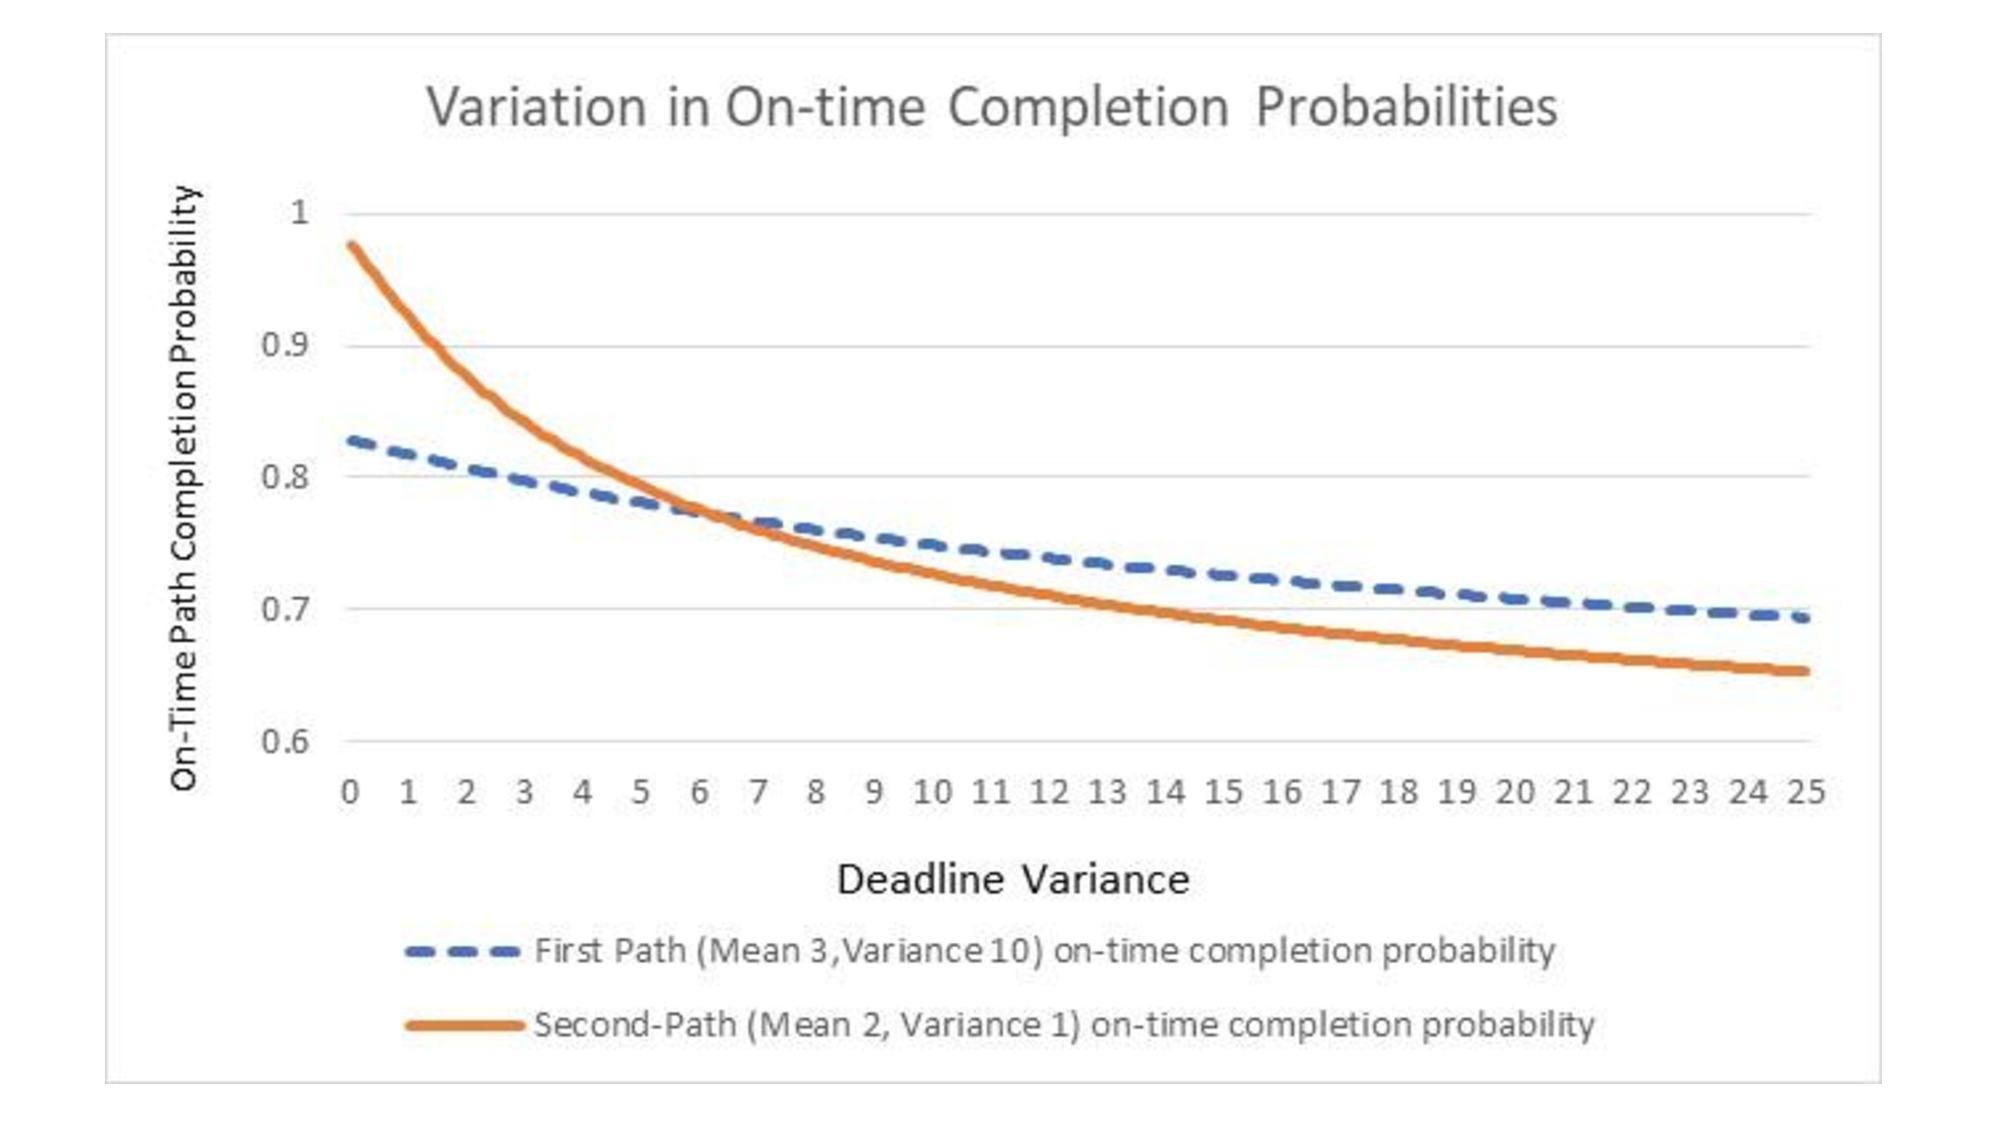
\includegraphics[scale=0.30]{uncertaindeadlinespath.pdf}
\caption{Variation of on-time path completion probability with deadline uncertainty}
\label{fig:p_vary_uncertainty}
\end{center}
\end{figure}
To prove that this is true in general for non-Gaussian distributions, suppose that the distribution of the standardized variable $\eta_i$ is the same as the distribution of the standardized variable $\eta_j$.   Consider paths $i$ and $j$ where path $i$ has higher actual schedule risk. Then
$$F_i(\frac{e_i}{\sqrt{v+v_i}}) \leq F_i (\frac{e_j}{\sqrt{v+v_j}}) \Longrightarrow \frac{e_i}{e_j} \leq \sqrt{\frac{v_i+v}{v_j+v}} $$
If schedule risk is ignored, then path $j$ will be perceived to have higher schedule risk whenever
$$\frac{e_i}{e_j} \geq \sqrt{\frac{v_i}{v_j}} $$
These conditions will both hold if
$$ \sqrt{\frac{v_i+v}{v_j+v}} \geq \frac{e_i}{e_j} \geq \sqrt{\frac{v_i}{v_j}} \Longrightarrow \frac{v_i+v}{v_j+v} \geq \frac{v_i}{v_j} \Longrightarrow 1+\frac{v}{v_i} \geq 1 + \frac{v}{v_j} \Longrightarrow v_j \geq v_i $$
Thus the manager who ignores deadline uncertainty will treat the low-variance path $i$ as having lower schedule risk even though its schedule risk is actually higher than high-variance path $j$. \par  If the manager's resources are constrained, the manager may incorrectly focus on controlling the schedule risk in the high-variance path at the expense of the low-variance path. Hence ignoring deadline uncertainty can lead to sub-optimal crashing of high variance paths. 
\subsection{Optimal crashing of a path}
Let $R$ be the reward if the project is completed on-time and let $c$ for each unit by which the path's mean completion time is reduced. Then the manager adjusts $e_i$ to $e^*_i$ to optimize
 $$R F(\frac{e^*_i}{\sqrt{v+v_i}}) - c (e^*_i-e_i) \propto
  F(\frac{e^*_i}{\sqrt{v+v_i}}) - \frac{c}{R} e^*_i $$
  Let $c^*=\frac{c}{R}$.
  Suppose $F$ is unimodal and continuous with probability density $f$ where $f'(z)$ is strictly decreasing for $z>0$.   Then since $e^*_i>0$, the objective function is concave and the optimal solution satisfies $$  f(\frac{e^*_i}{\sqrt{v+v_i}}) \frac{1}{\sqrt{v+v_i}} -c^* =0 $$
Since $f$ is strictly decreasing, there exists an $e_v>0$ for which
$$f(\frac{e_v}{\sqrt{v+v_i}}) =c^* \sqrt{v+v_i}   $$
The manager who recognizes requirement uncertainty sets $e^*_i=e_{v}$ and gets payoff
$$R^*= F(\frac{e_v}{\sqrt{v+v_i}}) - c^* e_v $$
while the manager who ignores requirement uncertainty sets $e^0_i=e_{0}$ and gets payoff
$$R^0=F(\frac{e_{0}}{\sqrt{v+v_i}}) - c^* e_0 $$
For this problem, it is also interesting to consider a third case of the manager who can complete eliminate uncertainty (perhaps with a idealized agile process which gathers perfect information about the client's deadline prior to making crashing decisions.) This manager likewise sets $e^*_i=e_0$.  But when the manager makes this crashing decision, the deadline uncertainty is actually zero and the manager's reward is
$$R^{PI}=F(\frac{e_0}{\sqrt{v_i}} )-c^* e_0 $$
which exceeds the reward from setting $e^*_i=e_0$ when the deadline uncertainty is non-zero.\par
The expected value of perfect information on deadline uncertainty, EVPI, is given by
$EVPI= R^{PI}-R^*$ while the expected value of including information on deadline uncertainty is
$EVIU=R^*-R^0$.   Hence one measure of the relative value of including uncertainty is   $$\frac{R^*-R^0}{R^{PI}-R^0}  
= \frac{EVIU}{EVIU + EVPI}   $$
where
$$R^*-R^0= F(\frac{e_v}{\sqrt{v+v_i}})-F(\frac{e_0}{\sqrt{v+v_i}})+c^*(e_0-e_v) $$
and
$$R^{PI}-R^0= F(\frac{e_0}{\sqrt{v_i}})-F(\frac{e_0}{\sqrt{v+v_i}}) 
$$
Figure \ref{fig:expect_reward} plots this measure for $c^*=.025,.05,.10$.  (This figure assumes the normal distribution where
$F'(z)=f(z)=\frac{\exp(-\frac{1}{2}z^2)}{\sqrt{2 \pi()}}$.) This percentage improvement increases as the relative cost of crashing, $c^*$, decreases.) 
\begin{figure}[ht]
\begin{center}
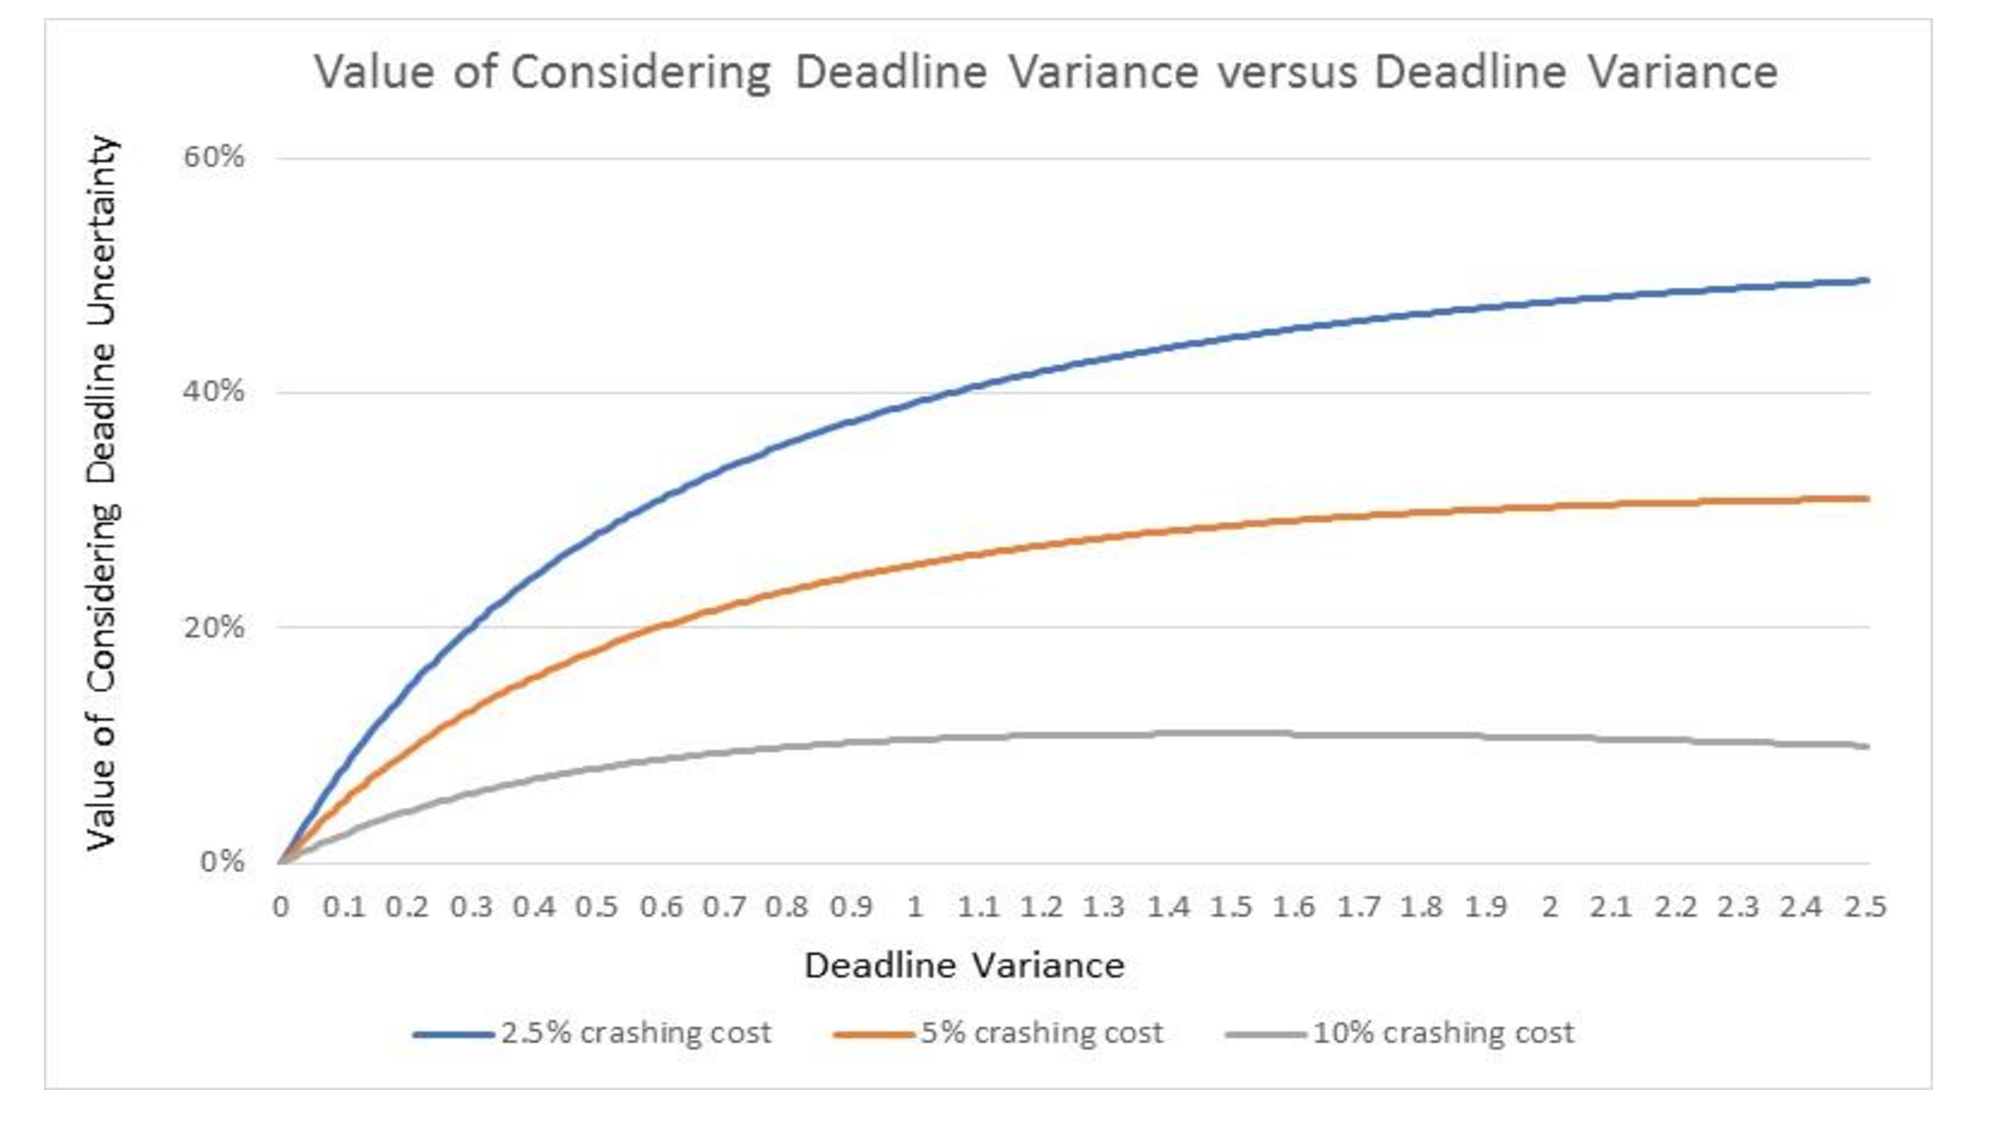
\includegraphics[scale=0.30]{ProjectMgtNewsvendor.pdf}
\caption{Variation of Expected Reward with deadline uncertainty}
\label{fig:expect_reward}
\end{center}
\end{figure}
For larger values of $c^*$, the measure is less than $0.5$ and the expected value of including uncertainty equals is less than the expected value of perfect information.   For smaller values of $c^*$, the measure exceeds $0.5$ and the expected value of including uncertainty exceeds the expected value of perfect information. \par
Note that 
$$
R^*-R^0 \approx F(\frac{e_0}{\sqrt{v_i}})
+ v f(\frac{e_0}{\sqrt{v_i}}) [\frac{e'_0}{\sqrt{v_i}} - \frac{e_0}{2 (v+v_i)^{3/2}}] - [F(\frac{e_0}{\sqrt{v_i}}) - v f( \frac{e_0}{\sqrt{v_i}})   (-\frac{e_0}{2 (v_i+v)^{3/2}}]  $$
which implies
$$
R^{**}-R^0= v f(\frac{e_0}{\sqrt{v_i}} )\frac{e'_0}
{\sqrt{v_i}} =
f(z^0)\frac{e'_0}
{\sqrt{v_i}}
$$

Likewise
$$R^{PI}-R^0=F(\frac{e_0}{\sqrt{v_i}}) -
F(\frac{e_0}{\sqrt{v+v_i}}) 
\approx - \frac{v}{2} f \frac{e_0}{(v+v_i)^{3/2}} 
$$
Substituting gives
$$\frac{R^*-R^0}{R^{PI}-R^0}
 \approx \frac{v \frac{e'_v}{\sqrt{v_i}} 
 f(z^0)}{\frac{v}{2} f(z_0) \frac{e_0}{v^{3/2}_i }  }
 =2 v_i \frac{e'_0}{e_0}
  $$
where $e'_0$ is obtained by implicitly differentiating 
$$f(\frac{e_v}{\sqrt{v+v_i}})=c^* \sqrt{v+v_i} \Longrightarrow f' [\frac{e'_v}{\sqrt{v_i+v}} - \frac{e_v}{2 (v+v_i)^{3/2}}] = \frac{c^*}{2 \sqrt{v+v_i}}  \Longrightarrow
e'_v = \frac{c^*}{2 f' \sqrt{v_i}} + \frac{e_v}{2 v_i} 
$$
Hence $\frac{e'_0}{e_0} = \frac{c^*}{2 f' e_0 \sqrt{v_i}} + \frac{1}{2 v_i}  $. 
Substituting gives
$$ \frac{R^*-R^0}{R^{PI}-R^0} \approx 
2 v_i  \frac{e'_0}{e_0} = \frac{c^*}{f' e_0} \sqrt{v_i} 
+1  $$ 
Since $f'<0$ for $e_i>0$, the ratio has a maximum value of one for $c^*$ small.

Figure \ref{fig:expect_reward} assumes a reward is associated with the on-time completion of a path (e.g., the critical path). But in reality, a reward is associated with the on-time completion of the project.  The probability of on-time completion of the project is typically less than the probability of on-time completion of any path in the project. Hence the reward associated with optimal crashing of any particular path is less than the reward associated with optimal crashing of the project (which leads to a larger value of  $c^*$.)\par
However this effect is complicated by the fact that crashing begins with one path but then switches to other paths as that one path becomes less critical.  The next section focuses on the implications of deadline uncertainty in project crashing.   Because of the greater complexity of the project, a subsequent section then uses simulation to estimate the impact of deadline uncertainty on projects.
\section{Project On-Time Completion Time}
\subsection{Overestimation of Completion Probability}
The probability of on-time completion for the project is the probability of on-time completion of every path in the project. Let $F(z_1,...z_k)$ be the multivariate cumulative probability of $\eta_1,...\eta_k$.  Sklar's Theorem (Nelsen, 2006) shows that that for every multivariate cumulative distribution $F(z_1,...z_k)$ with marginal distributions
$F_i(z_i), i=1...k$, there exists a multivariate copula function, $C(...)$ for which
$$F(z_1,...z_k)= C(F_1(z_1),...F_k(z_k)) =C(p_1,...p_k)$$
The copula function will reflect all the interdependencies between paths in the project.  The Frechet-Hoeffding bounds on the copula are
$$ \max(1-k+ \sum_{i=1}^k p_i, 0) \leq C(p_1,...p_k) \leq \min(p_1,...p_k)  $$
Since the average on-time completion probability is
$\hat{p}= \frac{\sum_{i=1}^k p_i}{k}$, the lower bound can be written as $\max(1-k(1-\hat{p}),0$ which will only be nonzero when the average schedule risk, $1-\hat{p}$ is less than $\frac{1}{k}$.   The upper bound on the on-time project completion probability becomes
  $$ \min(p_1,...p_k) \leq \min(F_1(0),...F_k(0)) \leq 0. 5  $$
which is less than $50\%$ when deadline variance approaches infinity. \par To develop a more explicit expression for how the project on-time completion time probability is underestimated when deadline uncertainty is ignored, consider a Taylor Series approximation of the project completion time probability about $v=0$.  Define
\begin{itemize}
    \item $p=C(p_1,...p_k)$ as the probability of on-time project completion 
    \item $p^0=C(p^0_1...p_k)$ as the calculated value of $P$ when deadline variance is ignored.
    \item $C_i=\frac{C}{\partial p_i}$ as the marginal change in project on-time completion probability when path i's marginal on-time completion probability is improved
    \item $C_i^0=\frac{\partial C}{\partial p_i}|_{v=0}$ 
    \item $C_{ij}=\frac{\partial^2 C}{\partial p_i \partial p_j}$ and $C^0_{ij}=
    \frac{\partial^2 C}{\partial p_i \partial p_j}|_{v=0} $ 
\end{itemize}
Then  
\begin{eqnarray*}
p &=& C(F_1(z_1),...F_k(z_k)) \approx C(p^0_1,...p^0_k) + v_0 [\sum_i C_i p'_i |_{v=0}]
+  \frac{1}{2} v^2 [\sum_{ij}  C_{ij} p'_i p'_j + \sum_i C_i p"_i]|_{v=0}   \\
&=& p^0 -\frac{1}{2}  \sum_i C^0_i f_i(z^0_i) z^0_i \frac{v}{v_i}  
+ \frac{1}{2} \sum_{ij} \frac{v^2}{v_iv_j} C^0_{ij} f_i(z^0_i)f_j(z^0_j) 
+ \sum_i \frac{v^2}{v^2_i} C^0_i
[\frac{1}{4} f'_i(z^0_i)  (z^0_i)^2 + 
\frac{3}{4} f_i(z^0_i) z^0_i]
\end{eqnarray*}
If we neglect the second-order term,  $$p^0-p \approx \frac{1}{2}  \sum_i C^0_i f_i(z^0_i) z^0_i \frac{v}{v_i}  $$
so that the overestimation in schedule risk, associated with ignoring deadline uncertainty, is proportional to a weighted sum of $\frac{v}{v_i}$ across all paths $i$.
\subsection{Crashing of Project Activities}
Number the activities in the project $m=1,....M$ and let $\pi_m$ be the amount of resources associated with crashing activity $m$.   In some cases, crashing of an activity significantly reduces its completion time.  In other cases, it introduces confusion into the project and may significantly increase its completion times. Let $x_m$ be the mean reduction in activity $m$'s completion time associated with spending $\pi_m$ on crashing. Let $\sigma^2_m$ be the mean increase in activity $m$'s variance associated with spending $\pi_m$ on crashing.  Since $x_m$ and $\sigma^2_m$ are both increasing functions of $\pi_m$, we can equivalently write $\sigma^2_m$ as a function of $x_m$ instead of $\pi_m$.   \par
Let $I_{jm}=1$ if activity $m$ is on path $j$ with $I_{jm}=0$ otherwise. If $e_j$ and $v_j$ are the mean and variance of $T-X_j$ prior to crashing, then reducing the mean duration of activity $m$ by $x_m$ for $m=1,...m$ leads to the following revised values of $e_j$ and $v_j$:
\begin{eqnarray*}
e^*_j &=& e_j+\sum_m x_m I_{jm}, j=1...k \\
v^*_j &=& v_j+\sum_m I_{jm} \sigma^2_m (x_m), j=1...k
\end{eqnarray*}
Consider: \\
\bf Assumption $3$: \rm The coefficient of variation of the uncertainty induced by crashing activity $m$ is some constant $s_m$ independent of $x_m$ 
\\ \bf Assumption 4: \rm  $\ln(p)$ is concave in $z_1,...z_k$. \\
Define  $w_j =\frac{\partial \log p}{\partial z_j} (v^*_j)^{-3/2}$.  As the Appendix shows, 
the optimal level of crashing for activity $m$ is $$x_m=\frac{\sum_j w_j I_{jm} v_j}{s^2_m \sum_j w_j I_{jm} e_j} \mbox{ with }
z^*_j = \frac{e_j+\sum_m I_{mj} x_m}{\sqrt{v_j+\sum_m I_{jm} (s_m x_m)^2}}  $$
which leads to the completion time probability
$C(F_1(z^*_1),...F_k(z^*_k))$.  Since $w_j$ is a function of $x_m$, there is typically no exact closed form expression for $x_m$. 
\par
The manager who ignores deadline uncertainty crashes activity $m$ by setting
$$x^0_m=\frac{\sum_j w^0_j I_{jm} (v_j-v)}{s^2_m \sum_j w^0_j I_{jm} e^0_j}  \mbox{ with }
z^0_j = \frac{e_j+\sum_m x^0_m I_{jm}}{\sqrt{v_j+\sum_m I_{jm} (s_m x^0_m)^2}}=
\frac{e^*_j+\sum_m (x^0_m-x_m) I_{jm}}{\sqrt{v^*_j+\sum_m I_{jm} [(s_m x^0_m)^2-(x_m)^2}}
$$
which leads to the completion time probability
$$C(F_1(\sqrt{\frac{v_1}{v_1+v}} z^0_1),...,F_k(\sqrt{\frac{v_k}{v_k+v}} z^0_k)) $$
Comparing the expected reduction in payoff from ignoring deadline uncertainty requires specification of the copula function $C$ which depends upon the project precedence density.  The next section will use a simulation of different project precedence densities to implicitly specify the copula and the optimal crashing levels $x_m$.
\section{Simulation Comparison of Alternate Approaches}
This section presents a designed experiment using a set of 1000 randomly simulated projects which a) demonstrates the importance of considering deadline uncertainty, and b) numerically compares different crashing strategies.

The crashing strategies evaluated are the conventional PERT approach, which ignores deadline uncertainty, and this paper's proposed approach (modified-PERT) which incorporates deadline uncertainty.
There is a trade-off between the ease of implementation and benefit of the proposed approach compared to that for more modelling intensive approaches.
Of course, if the project conforms exactly to the assumptions of the proposed approach, additional modelling efforts will not produce any benefit. 
To explore the usefulness of the proposed approach extended to other situations, this paper evaluates the effectiveness of these two crashing strategies.
As a reference, this paper also considers the effectiveness of the computationally intensive explicit enumeration algorithm (which is treated as an upper bound on the effectiveness of crashing). 
This greedy enumeration algorithm is used as a surrogate for formal optimization routines.
This comparison shows that the enumeration algorithm is only slightly superior to the proposed approach while the proposed approach is clearly superior to PERT. This minor difference between the enumeration and the modified-PERT means the choice between the two involves a tradeoff between the computational cost of this algorithm and the incremental value of its improvement.
\par
\subsection{Method}
We generate $1000$ projects with five to ten activities using Monte Carlo simulation\footnote{This code is available from **github link radacted for peer-review**}. (The number of activities was chosen to allow for interesting variations in project structure without leading to a computationally unmanageable number of paths.) The algorithm draws the number of activities and the probability of precedence from Uniform distributions (5,10) and (0.05,0.4) respectively. (Projects with few activities and/or low precedence density will have paths that do not share activities, while at the high end paths may share several -- and in some cases the majority of -- activities.) Project paths are then defined to be consistent with the precedence relationships between the activities. As this paper proposed, an activity representing the deadline was added to each path.  The mean completion time of the deadline was identified as the 90\% quantile of the critical path, and the coefficient of variation (CV), with which the variance was calculated, was systematically varied to compare between crashing strategies.
\par
The uniform distribution is again used to generate the mean ($U\approx(0,1)$) for each activity.  The CV of each activity was also drawn from a standard uniform distribution.  The mean completion time of a path is the sum of the mean duration of activities on that path. 
The mean slack of a path, i.e., the mean time by which it finishes ahead of schedule is the difference between the mean deadline and the path's mean completion time.   Activities are assumed independent so that the variance of a path's completion time is the sum of the variances of the activities along that path.   The variance of the path's slack is the sum of the variance of the deadline and the sum of the variance of the path's activities.
As activity completion times are assumed to be independent, the covariance between two paths is the sum of the variances of the activities shared by those paths. Note that the covariance between each path's slack will also include the variance of the deadline.  The covariance between paths, along with the standard deviation of each path, then specifies the correlation between each path.  
\par
The software R allows for the computation of the minimum of up to $1000$ Gaussian random variables (Genz et al., 2017).  The probability of the minimum being non-negative is the probability of all paths on the project finishing on-time (given the uncertainty in the deadline.) This equals the probability of the slack for every path being non-negative.

Each crashing strategy operates using a crashing reward function: $$\max R(v,d) = \Delta P(s|v,d) - c d$$ Where $\Delta P(s|v,d)$ is the change in probability of success given variance is considered or not ($v \in \{0,1\}$) and some level of crashing $d$. $c$ is the cost per unit of crashing.  

This program simulated one thousand projects. For each of these projects, the deadline coefficient of variation was varied, and the crashing rules applied. The crashing rules are
\begin{itemize}
\item crashing using the PERT algorithm. To identify the  activity to crash, PERT first identifies the critical path, i.e., the path with greatest mean completion time. The critical activity is the activity on the critical path with longest mean duration. The mean duration of this activity is reduced to maximize the reward function. If the critical path is still critical, then crashing moves to another activity on the critical path.  If the critical path is no longer critical, then crashing moves to another activity on the path which has become critical.  Crashing stops when additional crashing does not maximize the reward function. 
\item crashing with modified-PERT: To identify the activity to crash, our modifies PERT heuristic first calculates the univariate probability of each path exceeding the deadline. The activity with the largest mean on this critical path is selected to crash. As with the PERT algorithm, the mean is reduced subject to the reward function. Once the activity is crashed the algorithm repeats.   
\item crashing based on explicit enumeration: To identify the activity to crash, explicit enumeration considers completely crashing every activity to determine which would maximize on-time project completion. As before, the crashing first focused on the activity with greatest impact on project completion. Once this activity is identified, the reward function is used to determine the optimal amount of crashing. This is repeated until crashing no longer maximizes the reward function. While explicit enumeration is not feasible for larger networks, it provides an upper bound on what is possible with sophisticated optimization methods.
\end{itemize}

\begin{figure}[H]
\begin{center}
\begin{subfigure}[b]{0.85\linewidth}
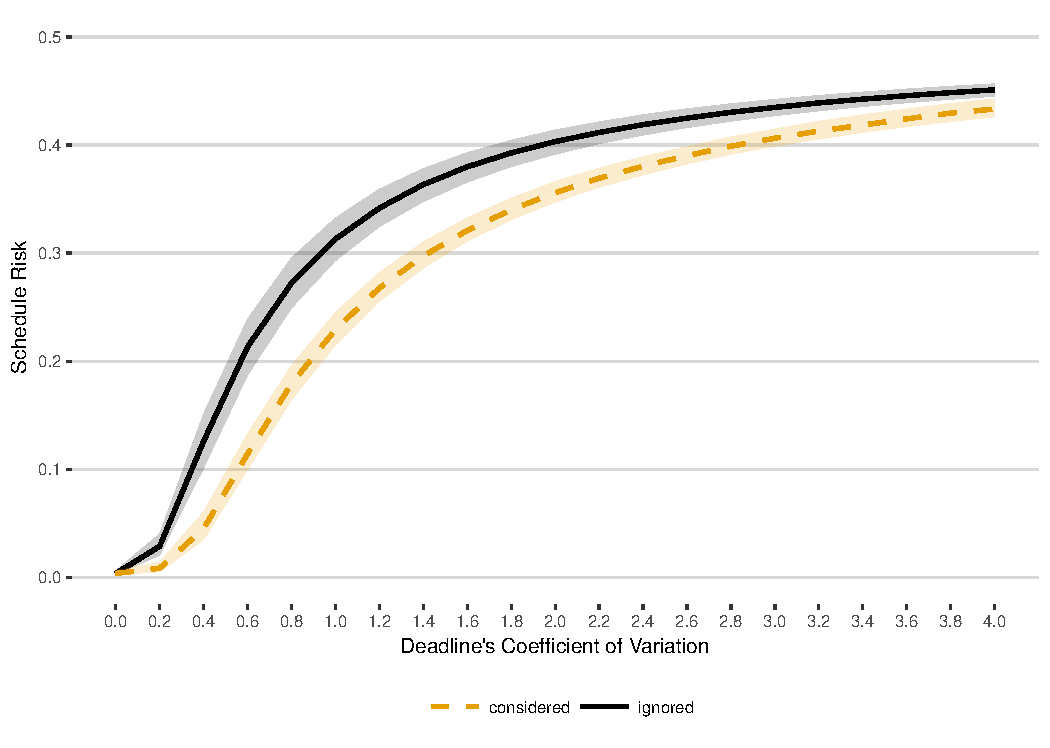
\includegraphics[width=\textwidth]{2018-07-24_CoV-vary_reward.pdf}
\caption{The median and 5\textsuperscript{th} and 95\textsuperscript{th} percentiles of the schedule risk when crashing paths with full enumeration considering and ignoring uncertainty. }
\label{fig:consider_uncertainty}
\end{subfigure}

\begin{subfigure}[t]{0.4\linewidth}
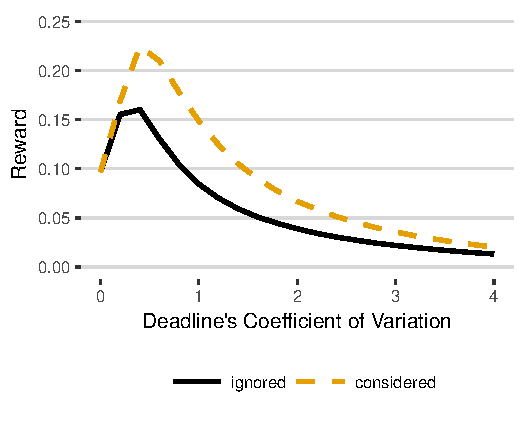
\includegraphics[width=\textwidth]{2018-07-24_CoV-vary_reward-mean.pdf}
\caption{The reward function when ignoring and considering deadline uncertainty.}
\label{fig:reward}
\end{subfigure}

\caption{Comparing the schedule risk of crashing strategies which ignore and consider deadline uncertainty on a simulation of 1000 simulated projects. Ignoring uncertainty leads to significantly higher schedule risk.}
\end{center}
\end{figure}




Figure \ref{fig:consider_uncertainty} presents the schedule risk for projects crashed using enumeration which considers and ignores deadline uncertainty. This shows the importance of considering deadline uncertainty given that the improvement in schedule risk can be up to 15\%. Figure \ref{fig:reward} presents the reward function for \ref{fig:consider_uncertainty}. 

Figure \ref{fig:crash_alternatives} shows the schedule risk for different crashing strategies. These results present the 5\textsuperscript{th} and 95\textsuperscript{th} percentiles from the 1000 projects, indicating PERT significantly under performs modified-PERT and enumeration when deadline uncertainty is non zero. The modified-PERT is only slightly different from the enumeration which provides managers a computationally and practically viable way of identifying near-optimal crashing that is robust to deadline uncertainty. As deadline uncertainty increases to be significantly greater than the activity uncertainties and paths, the results converge, indicating that crashing does little to improve probability of completion. 
    
Instead of simply focusing on mean performance (i.e. Figure \ref{fig:crash_alternatives}), Figures \ref{fig:cp_dif} compare the performance of modified PERT heuristic and PERT across all the simulation runs with 5\textsuperscript{th} and 95\textsuperscript{th} percentiles.  As this figure highlights, the modified PERT heuristic significantly outperforms PERT. Figure \ref{fig:brute_dif} similarly compares the modified PERT heuristic and explicit enumeration.   This figure shows that explicit enumeration is not significantly better than the modified-PERT heuristic. 
While explicit enumeration is not feasible for practical project networks, it does establish an upper bound on what might be possible with sophisticated optimization algorithms, both now and in the future.  These results suggest that the modified PERT heuristic, because of its simplicity, is an attractive alternative to more conventional optimization except for those projects where the value of marginal improvements in on-time project completion is very high. 

These results provide solid evidence of the value of this paper's proposed adjustment for deadline uncertainty.

  
\begin{figure}[H]
\begin{center}
\begin{subfigure}[b]{0.8\linewidth}
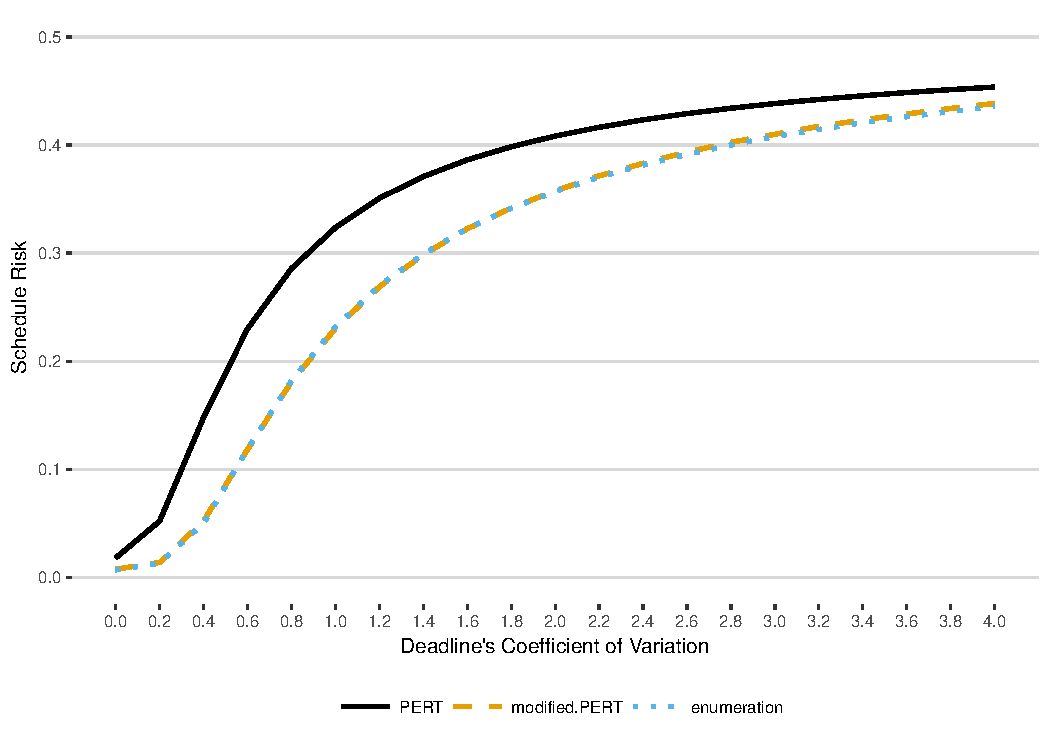
\includegraphics[width=\textwidth]{2018-07-25_CoV-vary_mean.pdf}
\caption{Mean probability of on-time completion with alternative crashing strategies as the deadline coefficient of variation changes.}
\label{fig:crash_alternatives}
\end{subfigure}
\begin{subfigure}[t]{0.35\linewidth}
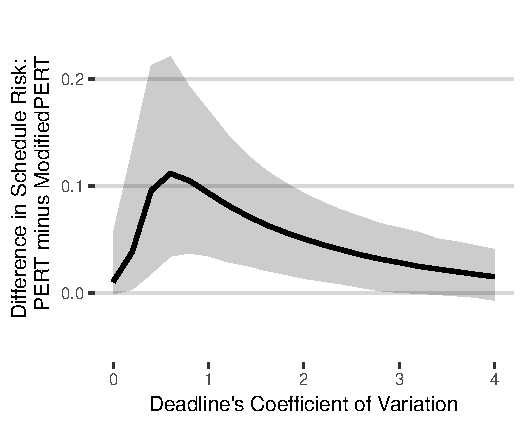
\includegraphics[width=\textwidth]{2018-07-25_critical.pdf}
\caption{The mean difference between PERT and modified-PERT crashing strategies.}
\label{fig:cp_dif}
\end{subfigure}
\begin{subfigure}[t]{0.35\linewidth}
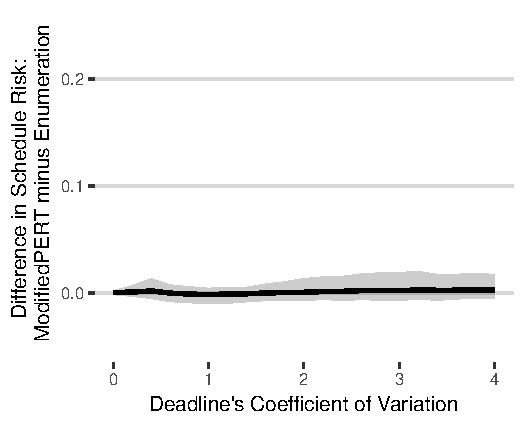
\includegraphics[width=\textwidth]{2018-07-25_brute.pdf}
\caption{The mean difference between modified-PERT and explicit the enumeration strategy}
\label{fig:brute_dif}
\end{subfigure}
\caption{Comparing the probability of on-time completion as the deadline's coefficient of variation changes for various crashing strategies used on a simulation of 1000 simulated projects. The lower plots display the 5\textsuperscript{th} and 95\textsuperscript{th} percentiles.}
\end{center}
\end{figure}


\section{Generality of this Approach}
This approach was designed to supplement those project management techniques which presume that the project deadline is fixed.  Our innovation is in showing how uncertain deadlines could be easily integrated into project management methods using a dummy activity.  The most common scheduling technique used in project management is PERT.  But PERT makes several unrealistic assumptions.  This section focuses on showing that our solution, and the benefits of our solution, are not contingent on the assumptions used in PERT.  
\subsection{The PERT Objective Function}
PERT focuses on maximizing the probability of finishing the project by the deadline.  But there are many other objectives e.g., the minimization of expected project completion time or more generally the maximization of the expected utility of project completion time.  The expected utility function (Castagoli and LiCalzi, 1996) can always be written as the cumulative distribution of some uncertain target.  As a result, maximizing an expected utility defined over project completion time is equivalent to maximizing the probability of completion time being less than some uncertain target.  Since the uncertainty in this uncertain target can be incorporated into the uncertainty in the deadline,  this paper's methodology for maximizing the probability of finishing by an uncertain deadline can likewise be used to maximize any expected utility function defined over project completion time.  So this approach allows for a very general set of objective functions.
\subsection{Generalizing to Non-normal Distributions}
  PERT implicitly assumes that the project completion time is normally distributed.  This assumption is invalid since the maximum of normal distributions cannot be normally distributed. However this paper's innovation of adding a complementary activity is unaffected by whatever distribution is assumed for the completion time of the paths through the project.  Furthermore the project simulations only make some simple easily modifiable assumptions about activity durations and make no assumptions about either path or project completion time distributions.  In calculating the bound on on-time completion probability, this paper did assume unimodal skewed distributions, with finite means and variances, for the completion time of paths. This assumption is consistent with a wide variety of non-normal distributions, including max-stable distributions like the Gumbel, reverse Weibull and Frechet.   \subsection{Generalizing to Resource-Based Scheduling}
PERT assumes each activity will start as soon as all precursor activities are finished.  But if the start of this new activity will monopolize equipment needed by an activity that starts later, starting each activity as soon as possible may delay the project's completion time.  Since this paper shows how our approach can improve resource-allocation decisions (like crashing), the proposed method is potentially useful in these more complex decisions.  \par
\subsection{Relaxing PERT's critical Path Assumption}
Finally PERT assumes project completion time is determined by the completion time of the critical path.  Since the proposed approach creates a complementary activity which starts after every activity is finished, the value of the proposed approach is unaffected by which path actually finishes last. \par

\section{Summary}
Many projects must be completed in the presence of uncertainty about when the stakeholder requires the project to be finished.    Conventional project management currently requires that the project manager assume a fixed required project completion time, until such time as it is formally modified by a change control process.   The sub-optimality of this approach to decision making is well-known.  As this paper shows, this deficiency can be corrected by simply supplementing the initial list of project activities with a fictitious dummy activity with the same uncertainty as currently exists in the deadline. The fixed deadline for the supplemented project is defined as the optimistic estimate for the original uncertain deadline.  Managing this supplemented project appropriately using standard methods of project management then appropriately accounts for the uncertainty in the deadline.\par
The paper then focused on establishing the benefits of this simple adjustment.  As the paper shows,  recognizing deadline uncertainty leads to more accurate (and less optimistic) estimates of on-time completion probability.  It also correctly identifies those paths (especially low-variance paths) with the largest schedule risk.  A second-order Taylor Series approximation can also be used to estimate how much ignoring deadline uncertainty overestimates a project's on-time completion probability. It leads to more informed crashing decisions which significantly improve the project's on-time completion probability.
\par
To quantify the benefits of the proposed approach, this paper presented a Monte Carlo simulation of a thousand projects comparing a PERT crashing rule, the modified PERT rule that recognizes deadline uncertainty and a near-optimal rule.   The simulation established that both the modified PERT rule and the near-optimal rule substantially outperformed PERT.  It also established that the near-optimal rule was only slightly better than modified PERT.  \par
The performance of the  near-optimal rule is potentially achievable with Resource Constrained Project Scheduling Problems (RCPSP, e.g., Brucker et al, 1999) and other formal optimization approaches.  But while technically better, these methods are harder for most project managers to use. Hence evaluating our approach versus the near-optimal approaches involves a cost/benefit analysis of how well our enhancement of PERT performs compared to more difficult, but higher performing, stochastic optimization methods.  In high-value applications, the higher performing methods may still be more attractive. But in the bulk of the more moderate-value applications of project management, the approach proposed in this paper is an attractive simpler alternative.  \par
In summary, the key contribution of this paper was to introduce the new
and somewhat counter-intuitive idea of recognizing the uncertainty in the project deadline by introducing an artificial activity.  In the context of project management, this way of recognizing deadline uncertainty requires only minimal changes in existing methodologies.  This paper introduced this idea and estimated its potential improvement in existing project management practices.
\begin{thebibliography}{10}
\bibitem{bbb} Brucker, P., A. Drexl, R. Mohring, K. Neumann, and E. Pesche (1999). Resource-constrained project scheduling: Notation, classification, models,
 and methods. {\em European Journal of Operational Research}. 112. 3-41
  \bibitem{a} Calhoun, K., R. Deckro, J. Moore, J. Chrissis and J. Van Hove. (2002). Planning and re-planning in project and production scheduling. {\em Omega.} 30, 155-170.
  \bibitem{b}	Chapman, C and S. Ward. (1997). {\em Project Risk Management: Processes, Techniques and Insights.} Wiley, New York
  \bibitem{c}	Clemen, R. (1996). {\em Making Hard Decisions.} 2nd ed. Duxbury Press, Belmont, MA.
  \bibitem{cc}  Creemers, S., B. De Reyck and R. Leus (2015). Project planning with alternative technologies in uncertain environments. {\em European Journal of Operational Research.} 242(2), 465-476.
  \bibitem{d}	Ding, C. and Y. Zhu.(2015). Two empirical uncertain Models for project scheduling problem. {\em Journal of the Operational Research Society.} 66, 1471-1480.
 \bibitem{e}	Elmaghraby, S. (2005). On the fallacy of averages in project risk management. {\em European Journal of Operational Research.} 165, 307-313.
 \bibitem{est}  Estevez-Fernandez, A. (2012).  A game theoretical approach to sharing penalties and rewards in projects. {\em European Journal of Operational Research.} 216(3), 647-657.
   \bibitem{f}	Golenko-Ginzburg, D. (1989). PERT assumptions revisited.{\em Omega} 17, 393-396.
  \bibitem{g}	Herroelen, W. and R. Leus (2005). Project scheduling under uncertainty: Survey and research potentials. {\em European Journal of Operational Research.} 165. 289-306.
  \bibitem{h}	Herroelen, W. and R. Leus (2003). The construction of stable project baseline schedules. {\em European Journal of Operational Research.} 156. 550-565.
  \bibitem{hh}  Hu, X., N. Cui, E. Demeulemeester, and L. Bie (2016). Incorporation of activity sensitivity measures into buffer management to manage project schedule risk. {\em European Journal of Operational Research}, 249(2), 717-727.
  \bibitem{j}	Huemann, M., R. Turner and A. Keegan (2007). Managing human resources in the project-oriented company. In Morris, P and J. Pinto. {\em The Wiley Guide to Project Organization and Project Management Competencies.} John Wiley \& Sons: Hoboken, New Jersey
  \bibitem{k}	Kamburkowski, J. (1996). New validations of PERT times.  {\em Omega}, 25(3) 323-328.
  \bibitem{l}	Keisler, J. and R. Bordley. (2015). Project management decisions with uncertain targets. {\em Decision Analysis.} 12, 1, 15-28.
  \bibitem{keefer} Keefer, D. and W. Verdini (1993). Better estimation of PERT activity time parameters. {\em Management Science.} 39, 9, 1086-1091.
  \bibitem{m}	Kerzner, H.  (2009)  {\em Project Management: A Systems Approach to Planning, Scheduling and Controlling.} John Wiley \& Sons: Hoboken, New Jersey
  \bibitem{n}	Khodakarami, V., N. Fenton and M. Neil. (2007). Project scheduling: Improved approach to incorporate uncertainty using Bayesian networks. {\em Project Management Journal.} 38(2),  39-49.
  \bibitem{o}	Klastorin, Ted (2003). {\em Project Management: Tools and Trade-offs} (3rd ed.). John Wiley \& Sons: Hoboken, New Jersey.
\bibitem{lr}  Levin, J., and Fox, J.A. (2003), {\em Elementary Statistics in Social Research}, 9th ed., Boston: Allyn and Bacon.
  \bibitem{p}	Maylor, H., R. Vidgen and S. Carver (2008). Managerial complexity in project-based operations: A grounded model and its implications for practice.  {\em Project Management Journal.} 39(S1), S15-S26.
  \bibitem{r}	Meredith, J., S. Mantel (1995). {\em Project Management: A Managerial Approach.} John Wiley and Sons, Hoboken: New Jersey
  \bibitem{s}	Miller, R. (1963). {\em Schedule, Cost and Profit Control with PERT.} McGraw-Hill, New
              York.
  \bibitem{t} Morgan, M. and M. Henrion (1992). {\em Uncertainty: A Guide to Dealing with Uncertainty in
  Quantitative Risk and Policy Analysis.}  Cambridge University Press:Cambridge, U.K.
  \bibitem{nels} Nelsen, R. (2006). {\em An Introduction to Copulas}. Springer Series in Statistics.
  \bibitem{neu}  Neumann, J. and J. Zimmerman (1999).  Resource leveling for projects with schedule-dependent windows.  {\em European Journal of Operational Research.}  117(3), 591-606.
  \bibitem{tt} Pérez, J. G., M.Martín, C. García and M. Granero (2016). Project management under uncertainty beyond beta: The generalized bicubic distribution. {\em Operations Research Perspectives} 3, 67-76.
  \bibitem{u} Pich, M. ,C.Loch and A. DeMeyer. (2002). On uncertainty, ambiguity, and
  complexity in project management. {\em Management Science}, 1008-1023, 48,8
  \bibitem{v} Project Management Institute (2013). {\em A Guide to the Project Management Body of
  Knowledge} (5th ed.). Project Management Institute.
  \bibitem{w} Schwaber, K.  (2004). {\em Agile Project Management with SCRUM.} Microsoft Press,
           Redmond, Washington
  \bibitem{x} Schwindt, C. (2005). {\em Resource Allocation in Project Management.} Springer: New York
  \bibitem{y} Sculli, D. (1989). A historical note on PERT times. {\em Omega} 17(2), 195-196.
  \bibitem{z} Vanhoucke, M. (2013). {\em Project Management with Dynamic Scheduling.} Springer, New
          York.
  \bibitem{ab} Ward, S. and C. Chapman.(2003). Transforming project risk management into project
          uncertainty management. {\em International Journal of Project Management}, 21, 97–105
  \bibitem{ac} Zafra-Cabeza, A., M. Ridao and E. Camacho. (2008). Using a risk-based approach to
         project scheduling: A case illustration from semiconductor manufacturing. {\em European
        Journal of Operational Research.} 190, 708-723.
  \bibitem{genz} Genz, A., F. Bretz, T. Miwa, X. Mi, F. Leisch, F. Scheipl, and T. Hothorn (2017).
  mvtnorm: Multivariate Normal and t Distributions. R package version 1.0-6. URL
  http://CRAN.R-project.org/package=mvtnorm
  \end{thebibliography}
  \section{Appendix }
  \subsection{First-Order Conditions}
  The first-order Kuhn-Tucker conditions for $x_1,...x_M$ are
$$\frac{\partial \log p}{\partial x_m} = \sum_{j=1}^k \frac{\partial \log p}{\partial z_j} 
\frac{\partial z_j}{\partial x_m} =0  , m=1,...M $$
where
$$ \frac{\partial z_j}{\partial x_m} = \frac{1}{\sqrt{v^*_j}} \frac{\partial e^*_j}{\partial x_m}-  
\frac{1}{2} e^*_j v_j^{-3/2} \frac{\partial v^*_j}{\partial x_m} = (v^*_j)^{-3/2} [v^*_j I_{jm} -   \frac{1}{2} e^*_j  \frac{\partial v^*_j}{\partial x_m}]  $$
Defining $w_j =\frac{\partial \log p}{\partial z_j} (v^*_j)^{-3/2}$ allows the Kuhn-Tucker condition to be written as
$$ \sum_j w_j [v^*_j I_{jm} -   \frac{1}{2} e^*_j  \frac{\partial v^*_j}{\partial x_m}] =0 $$
To simplify this expression, assume: \\
\bf Assumption $2$: \rm The coefficient of variation of the uncertainty induced by crashing activity $m$ is some constant $s_m$ independent of $x_m$ \\ 
Then 
$\frac{\sigma_m}{x_m}=s_m$, $\sigma^2_m=x^2_m s^2_m$ and $\frac{\partial v^*_j}{\partial x_m} = 2 x_m I_{jm} s^2_m$.  
Then
\begin{eqnarray*}
 \frac{\partial z_j}{\partial x_m} &=& (v^*_j)^{-3/2} [v^*_j I_{jm} -   \frac{1}{2} e^*_j  \frac{\partial v^*_j}{\partial x_m}] \\
  &=& (v^*_j)^{-3/2} [I_{jm} v^*_j-  e^*_j I_{jm} x_m s^2_m ]
\\ &=&
(v^*_j)^{-3/2}I_{jm} [v_j +  \sum_m I_{mj} x^2_m s^2_m -  (e_j + \sum_m I_{mj} x_m)  x_m s^2_m)]  \\
&=& (v^*_j)^{-3/2} I_{jm} [v_j-x_m s^2_m e_j]  
\end{eqnarray*}
Then $$\frac{\partial \ln p}{\partial x_m} =
\sum_{j=1}^k \frac{\partial \log p}{\partial z_j} 
\frac{\partial z_j}{\partial x_m} = \sum_j w_j I_{jm} [v_j-x_m s^2_m e_j] $$
which equals zero for the $x_m$ satisfying the first-order conditions.\subsection{Verifying Second-Order Conditions} 
To ensure the first-order conditions define an optimum, assume:
\\ \bf Assumption 4: \rm  $\ln(p)$ is concave in $z_1,...z_k$. \\
 This assumption will be true for log-concave densities like the normal distribution, extreme value distribution, the Laplace distribution, the logistics distribution, the uniform and exponential distribution as well as for many other distributions whose density is not log-concave (or are only log-concave for certain parameter settings.). Then
\\ Proposition: \rm Given the previous assumptions, $\ln(p)$ is concave in
$x_1,...x_m$ \\
 \bf Proof: \rm Since $\ln(p)$ is concave in $z_1,...z_k$, the Proposition will be proven if the Hessian matrix $\frac{\partial^2 z_j}{\partial x_{m_1} \partial x_{m_2}} \geq 0$, can be shown to be negative definite.   Define 
$A_{jm_1}=[v_j - x_{m_1} s^2_m e_j] $ so that $\frac{\partial z_j}{\partial x_{m_1}} = (v^*_j)^{-3/2} I_{jm_1} A_{j,m_1} $.  Then
\begin{eqnarray*}
\frac{\partial^2 z_j}{\partial x_{m_1} \partial x_{m_2}} &=& 
-\frac{3}{2} (v^*_j)^{-5/2} I_{jm_1} \frac{\partial v^*_j}{\partial x_{m2}} A_{jm_1}
-  (v^*_j)^{-3/2} I_{jm_1} \frac{\partial x_{m_1}}{\partial x_{m_2}} s^2_{m_1} e_j\\
&=& -3 (v^*_j)^{-5/2} I_{jm_1} I_{jm_2} x_{m_2} s^2_{m_2}) A_{jm_1}
-  (v^*_j)^{-3/2} \frac{\partial x_{m_1}}{\partial x_{m_2}} s^2_{m_1} e_j
\end{eqnarray*} Note that for $m_1=m_2$, this component of the Hessian is negative.  For $m_1 \neq m_2$, this component of the Hessian is  proportional to $A_{jm_1}$ where the first-order conditions imply 
$\sum_j w_j A_{jm_1}=0$ for every $m_1$.  
\subsection{Optimal Solution}
Solving the 
first-order Kuhn-Tucker conditions gives $$x_m=\frac{\sum_j w_j I_{jm} v_j}{s^2_m \sum_j w_j I_{jm} e_j} \mbox{ with }
z_j = \frac{e^*_j}{\sqrt{v^*_j}}  $$
where $$e^*_j=e_j+\sum_m I_{mj} x_m \mbox{ and }
v^*_j=v_j+\sum_m I_{jm} (s_m x_m)^2
$$
which leads to the completion time probability
$C(F_1(z_1),...F_k(z_k))$. 
\par
The manager who ignores deadline uncertainty crashes activity $m$ by setting
$$x^0_m=\frac{\sum_j w^0_j I_{jm} (v_j-v)}{s^2_m \sum_j w^0_j I_{jm} e^0_j}  \mbox{ with }
z^0_j = \frac{e_j+\sum_m x^0_m I_{jm}}{\sqrt{v_j+\sum_m I_{jm} (s_m x^0_m)^2}}=
\frac{e^*_j+\sum_m (x^0_m-x_m) I_{jm}}{\sqrt{v^*_j+\sum_m I_{jm} [(s_m x^0_m)^2-(x_m)^2}}
$$
which leads to the completion time probability
$$C(F_1(\sqrt{\frac{v_1}{v_1+v}} z^0_1),...,F_k(\sqrt{\frac{v_k}{v_k+v}} z^0_k)) $$
\end{document}
